% Koko
\documentclass[blue,normal,cn]{elegantnote}
\usepackage{array}
\usepackage{courier}
\usepackage{xcolor}
\usepackage{zhnumber}
\usepackage{ulem}
\usepackage{float}

\definecolor{ans}{RGB}{230, 74, 25}

\definecolor{light-gray}{gray}{0.95}
\newcommand{\code}[1]{\colorbox{light-gray}{\texttt{#1}}}
\newfontfamily\courier{Courier New}
\lstset{linewidth=1.1\textwidth,
	numbers=left,
	basicstyle=\small\courier,
	numberstyle=\tiny\courier,
	keywordstyle=\color{blue}\courier,
	commentstyle=\it\color[cmyk]{1,0,1,0}\courier, 
	stringstyle=\it\color[RGB]{128,0,0}\courier,
	frame=single,
	backgroundcolor=\color[RGB]{245,245,244},
	breaklines,
	extendedchars=false, 
	xleftmargin=2em,xrightmargin=2em, aboveskip=1em,
	tabsize=4, 
	showspaces=false
	basicstyle=\small\courier
}
\title{实验 5:指令调度与延迟分支}
\version{$\aleph$}
\date{\zhtoday}

\begin{document}
\author{
  \begin{tabular}[t]{c}
    于海鑫 \\
    2017211240
  \end{tabular}
}
\maketitle

\section{实验目的}
\begin{enumerate}
  \item 加深对指令调度技术的理解
  \item 加深对延迟分支技术的理解
  \item 熟练账务用指令调度技术解决流水线中的数据冲突的方法
  \item 进一步理解指令调度技术对 CPU 性能的改进
  \item 进一步理解延迟分支技术对 CPU 性能的改进
\end{enumerate}

\section{实验平台}

实验平台采用指令级和流水线操作级模拟器 \code{MIPSsim}。

\section{实验内容和步骤}

\begin{enumerate}[wide=0pt, listparindent=2em, parsep=0pt]
  \item 启动 MIPSsim(用鼠标双击 MIPSsim.exe)。
  \item 根据实验 2 的相关知识中关于流水线各段操作的描述,进一步理解流水线窗口中各段的功能,掌握各流水线寄存器的含义(双击各段,就可以看到各流水线寄存器中的内容)。
  \item 选择“配置” $\rightarrow$ “流水方式”选项,使模拟器工作在流水方式下
  \item 用指令调度技术解决流水线中的结构冲突与数据冲突:

        \begin{itemize}[leftmargin=3em, listparindent=2em, parsep=0pt]
          \item 启动 MIPSsim。
          \item 用 MIPSsim 的 “文件” $\rightarrow$ “载入程序”选项来加载 \code{schedule.s}(在模拟器所在文件夹下的“样例程序”文件夹中)。
          \item 关闭定向功能,这是通过“配置“ $\rightarrow$ ”定向“选项来实现的。
          \item  执行所载入的程序,通过查看统计数据和时钟周期图,找出并记录程序执行过程中各种冲突发生的次数,发生冲突的指令组合以及程序执行的总时钟周期数。

                \textcolor{ans}{
                  \begin{itemize}[leftmargin=3em, listparindent=2em, parsep=0pt]
                    \item RAW停顿:16
                    \item 自陷停顿:1
                    \item 发生冲突的指令组合:
                          \begin{itemize}[leftmargin=3em]
                            \item LW \$r2,0(\$r1) 和 ADD \$r4,\$r0,\$r2
                            \item ADD \$r4,\$r0,\$r2 和 SW \$r4,0(\$r1)
                            \item SW \$r4,0(\$r1) 和 LW \$r6,4(\$r1)
                            \item ADD \$r8,\$r6,\$r1 和 MUL \$r12,\$r10,\$r1
                            \item ADD \$r16,\$r12,\$r1 和 ADD \$r18,\$r16,\$r1
                            \item ADD \$r18,\$r16,\$r1 和 SW \$r18,16(\$r1)
                            \item SW \$r18,16(\$r1) 和 LW \$r20 8(\$r1)
                            \item MUL \$r22,\$r20,\$r14 和 MUL \$r24,\$r26,\$r14
                          \end{itemize}
                  \end{itemize}
                }
                \textcolor{ans}{总执行周期:33}

                \textcolor{ans}{运行报告:}
                \begin{lstlisting}
  汇总:
    执行周期总数:33
    ID段执行了15条指令

  硬件配置:
    内存容量:4096 B
    加法器个数:1		执行时间(周期数):6
    乘法器个数:1		执行时间(周期数)7		
    除法器个数:1		执行时间(周期数)10		
    定向机制:不采用

  停顿(周期数):
    RAW停顿:16		占周期总数的百分比:48.48485%
    其中:
      load停顿:6		占所有RAW停顿的百分比:37.5%
      浮点停顿:0		占所有RAW停顿的百分比:0%
    WAW停顿:0		占周期总数的百分比:0%
    结构停顿:0		占周期总数的百分比:0%
    控制停顿:0		占周期总数的百分比:0%
    自陷停顿:1		占周期总数的百分比:3.030303%
    停顿周期总数:17	占周期总数的百分比:51.51515%

  分支指令:
    指令条数:0		占指令总数的百分比:0%
    其中:
      分支成功:0		占分支指令数的百分比:0%
      分支失败:0		占分支指令数的百分比:0%

  load/store指令:
    指令条数:5		占指令总数的百分比:33.33333%
    其中:
      load:3		占load/store指令数的百分比:60%
      store:2		占load/store指令数的百分比:40%

  浮点指令:
    指令条数:0		占指令总数的百分比:0%
    其中:
      加法:0		占浮点指令数的百分比:0%
      乘法:0		占浮点指令数的百分比:0%
      除法:0		占浮点指令数的百分比:0%

  自陷指令:
    指令条数:1		占指令总数的百分比:6.666667%
\end{lstlisting}

                \textcolor{ans}{时钟周期图:}
                \begin{figure}[H]
                  \centering
                  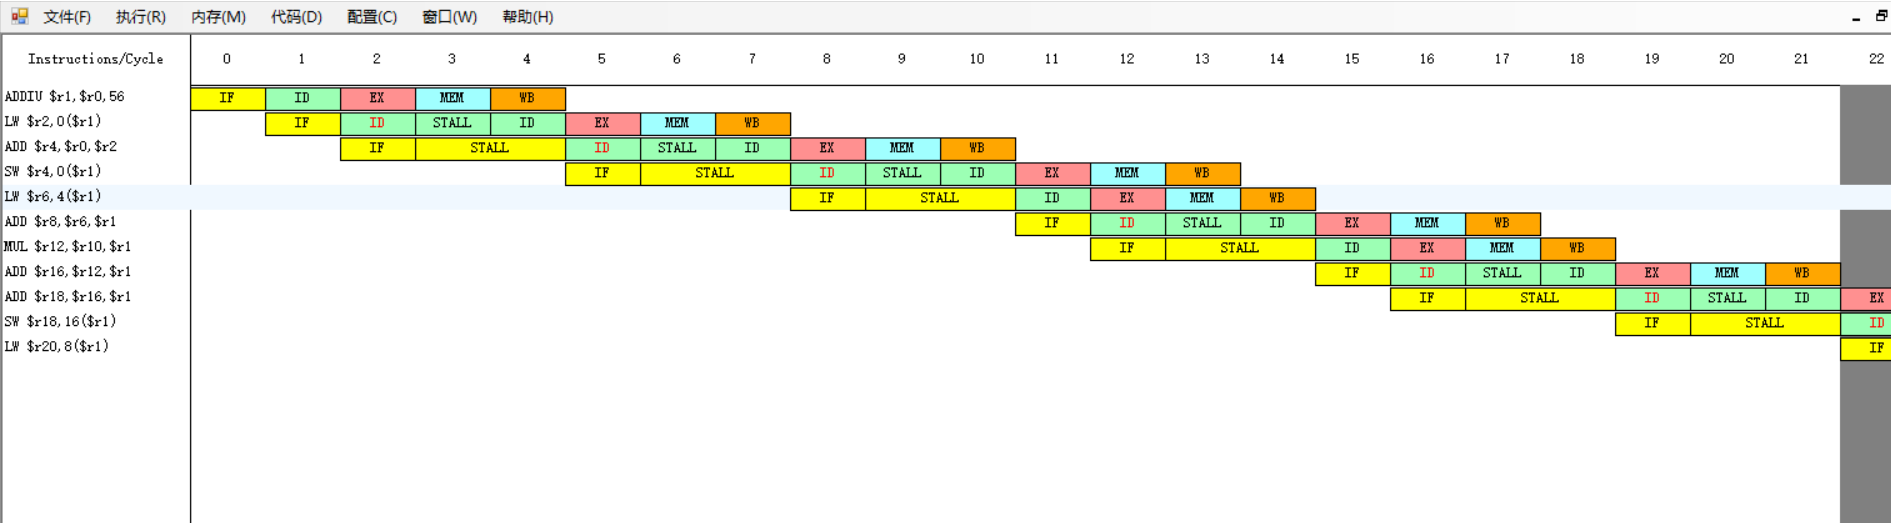
\includegraphics[width=.8\textwidth]{fig/schedule.png}
                  \caption{时钟周期图}
                \end{figure}

          \item 自己采用调度技术对程序进行指令调度,消除冲突(自己修改源程序)。将调度(修改)后的程序重新命名为 \code{afer-schedule.s}。(注意:调度方法灵活多样,在保证程序正确性的前提下自己随意调度,尽量减少冲突即可,不要求要达到最优。)

                \textcolor{ans}{优化后的程序:}

                \lstinputlisting{after-schedule.s}

          \item  载入 \code{afer-schedule.s},执行该程序,观察程序在流水线中的执行情况,记录程序执行的总时钟周期数。

                \textcolor{ans}{总执行周期:18}

                \textcolor{ans}{运行情况:}
                \begin{lstlisting}
  汇总:
    执行周期总数:18
    ID段执行了15条指令

  硬件配置:
    内存容量:4096 B
    加法器个数:1		执行时间(周期数):6
    乘法器个数:1		执行时间(周期数)7		
    除法器个数:1		执行时间(周期数)10		
    定向机制:不采用

  停顿(周期数):
    RAW停顿:1		占周期总数的百分比:5.555555%
    其中:
      load停顿:0		占所有RAW停顿的百分比:0%
      浮点停顿:0		占所有RAW停顿的百分比:0%
    WAW停顿:0		占周期总数的百分比:0%
    结构停顿:0		占周期总数的百分比:0%
    控制停顿:0		占周期总数的百分比:0%
    自陷停顿:1		占周期总数的百分比:5.555555%
    停顿周期总数:2	占周期总数的百分比:11.11111%

  分支指令:
    指令条数:0		占指令总数的百分比:0%
    其中:
      分支成功:0		占分支指令数的百分比:0%
      分支失败:0		占分支指令数的百分比:0%

  load/store指令:
    指令条数:5		占指令总数的百分比:33.33333%
    其中:
      load:3		占load/store指令数的百分比:60%
      store:2		占load/store指令数的百分比:40%

  浮点指令:
    指令条数:0		占指令总数的百分比:0%
    其中:
      加法:0		占浮点指令数的百分比:0%
      乘法:0		占浮点指令数的百分比:0%
      除法:0		占浮点指令数的百分比:0%

  自陷指令:
    指令条数:1		占指令总数的百分比:6.666667%
\end{lstlisting}

                \textcolor{ans}{时钟周期图:}
                \begin{figure}[H]
                  \centering
                  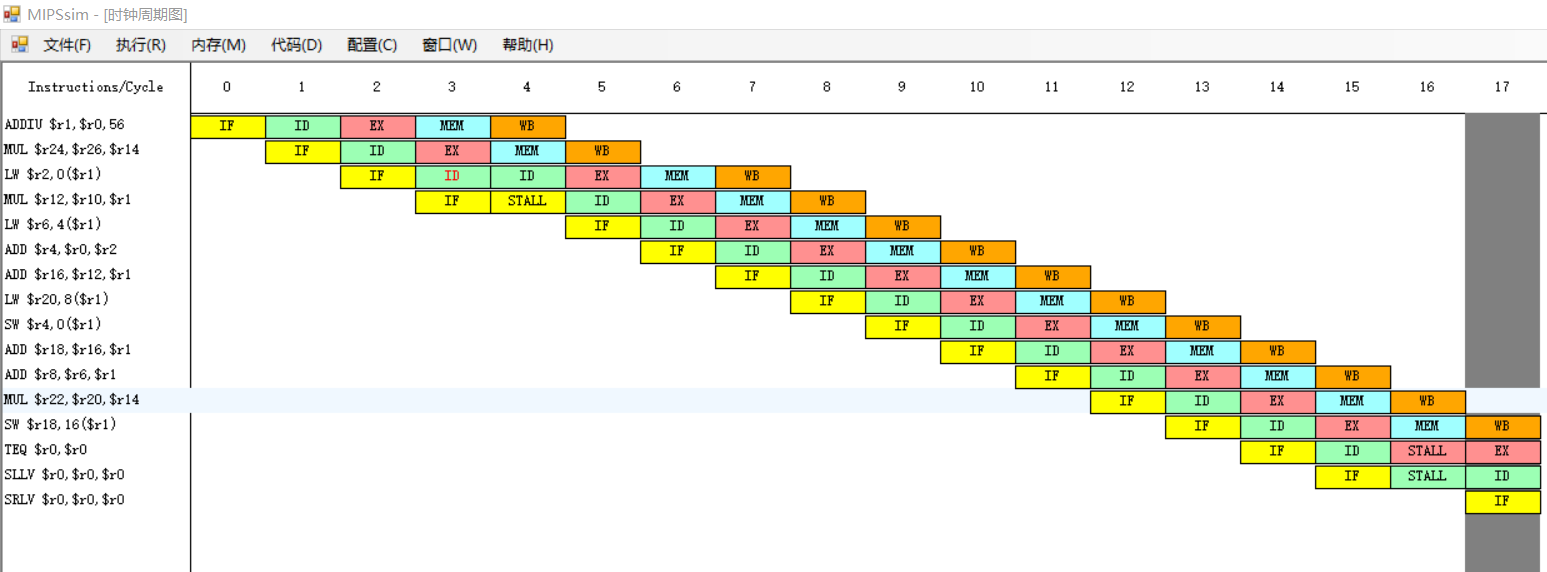
\includegraphics[width=.8\textwidth]{fig/after-schedule.png}
                  \caption{时钟周期图}
                \end{figure}

          \item 比较调度前和调度后的性能,论述指令调度对提高 CPU 性能的作用。

                \textcolor{ans}{调度前的执行周期为 33,调度后的执行周期数为 18。}

                \textcolor{ans}{指令调度可以消除部分的数据冲突,通过使用指令调度提高了CPU的使用率,大大减少了指令冲突的次数,提高了CPU性能。}


        \end{itemize}

  \item 用延迟分支技术减少分支指令对性能的影响:

        \begin{itemize}[leftmargin=3em, listparindent=2em, parsep=0pt]
          \item 在 MIPSsim 中载入 branch.s 样例程序(在本模拟器目录的“样例程序”文件夹中。
          \item 关闭延迟分支功能。这是通过在“配置” $\rightarrow$ “延迟槽”选项来实现的。
          \item 执行该程序,观察并记录发生分支延迟的时刻,记录该程序执行的总时钟周期数。

                \textcolor{ans}{总执行周期:38}

                \textcolor{ans}{第 14,29 周期发生了分支延迟}
                \textcolor{ans}{运行情况:}
                \begin{lstlisting}
  汇总:
    执行周期总数:38
    ID段执行了18条指令

  硬件配置:
    内存容量:4096 B
    加法器个数:1		执行时间(周期数):6
    乘法器个数:1		执行时间(周期数)7		
    除法器个数:1		执行时间(周期数)10		
    定向机制:不采用

  停顿(周期数):
    RAW停顿:16		占周期总数的百分比:42.10526%
    其中:
      load停顿:4		占所有RAW停顿的百分比:25%
      浮点停顿:0		占所有RAW停顿的百分比:0%
    WAW停顿:0		占周期总数的百分比:0%
    结构停顿:0		占周期总数的百分比:0%
    控制停顿:2		占周期总数的百分比:5.263158%
    自陷停顿:1		占周期总数的百分比:2.631579%
    停顿周期总数:19	占周期总数的百分比:50%

  分支指令:
    指令条数:2		占指令总数的百分比:11.11111%
    其中:
      分支成功:1		占分支指令数的百分比:50%
      分支失败:1		占分支指令数的百分比:50%

  load/store指令:
    指令条数:4		占指令总数的百分比:22.22222%
    其中:
      load:2		占load/store指令数的百分比:50%
      store:2		占load/store指令数的百分比:50%

  浮点指令:
    指令条数:0		占指令总数的百分比:0%
    其中:
      加法:0		占浮点指令数的百分比:0%
      乘法:0		占浮点指令数的百分比:0%
      除法:0		占浮点指令数的百分比:0%

  自陷指令:
    指令条数:1		占指令总数的百分比:5.555555%
\end{lstlisting}

                \textcolor{ans}{时钟周期图:}
                \begin{figure}[H]
                  \centering
                  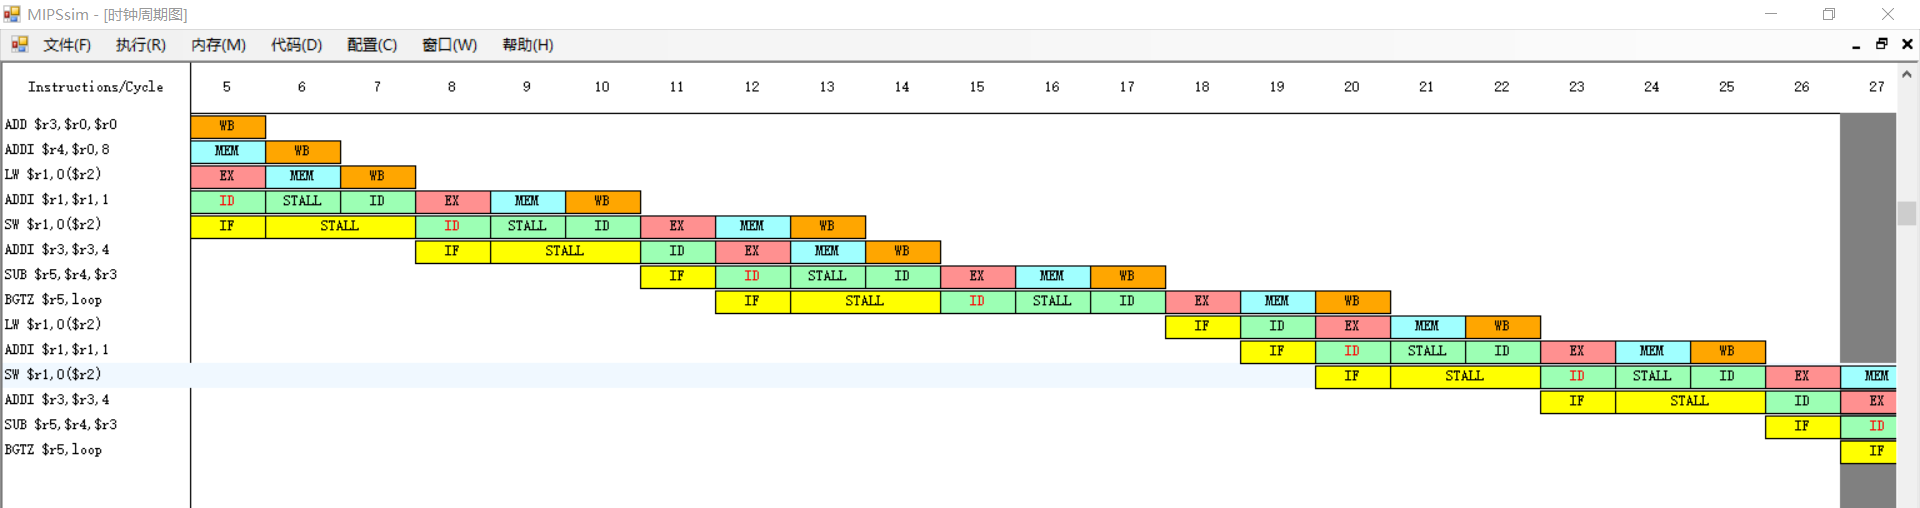
\includegraphics[width=.8\textwidth]{fig/branch.png}
                  \caption{时钟周期图}
                \end{figure}

          \item  假设延迟槽为一个,自己对 branch.s 程序进行指令调度(自己修改源程序),将调度后的程序重新命名为 delayed-branch.s。

                \textcolor{ans}{优化后的程序:}

                \lstinputlisting{delayed-branch.s}

          \item 载入 delayed-branch.s,打开延迟分支功能,执行该程序,观察其时钟周期图,记录程序执行的总时钟周期数。
                \textcolor{ans}{总执行周期:31}

                \textcolor{ans}{运行情况:}
                \begin{lstlisting}
  汇总:
    执行周期总数:31
    ID段执行了19条指令

  硬件配置:
    内存容量:4096 B
    加法器个数:1		执行时间(周期数):6
    乘法器个数:1		执行时间(周期数)7		
    除法器个数:1		执行时间(周期数)10		
    定向机制:不采用

  停顿(周期数):
    RAW停顿:10		占周期总数的百分比:32.25806%
    其中:
      load停顿:4		占所有RAW停顿的百分比:40%
      浮点停顿:0		占所有RAW停顿的百分比:0%
    WAW停顿:0		占周期总数的百分比:0%
    结构停顿:0		占周期总数的百分比:0%
    控制停顿:0		占周期总数的百分比:0%
    自陷停顿:1		占周期总数的百分比:3.225806%
    停顿周期总数:11	占周期总数的百分比:35.48387%

  分支指令:
    指令条数:2		占指令总数的百分比:10.52632%
    其中:
      分支成功:1		占分支指令数的百分比:50%
      分支失败:1		占分支指令数的百分比:50%

  load/store指令:
    指令条数:5		占指令总数的百分比:26.31579%
    其中:
      load:3		占load/store指令数的百分比:60%
      store:2		占load/store指令数的百分比:40%

  浮点指令:
    指令条数:0		占指令总数的百分比:0%
    其中:
      加法:0		占浮点指令数的百分比:0%
      乘法:0		占浮点指令数的百分比:0%
      除法:0		占浮点指令数的百分比:0%

  自陷指令:
    指令条数:1		占指令总数的百分比:5.263158%

\end{lstlisting}

                \textcolor{ans}{时钟周期图:}
                \begin{figure}[H]
                  \centering
                  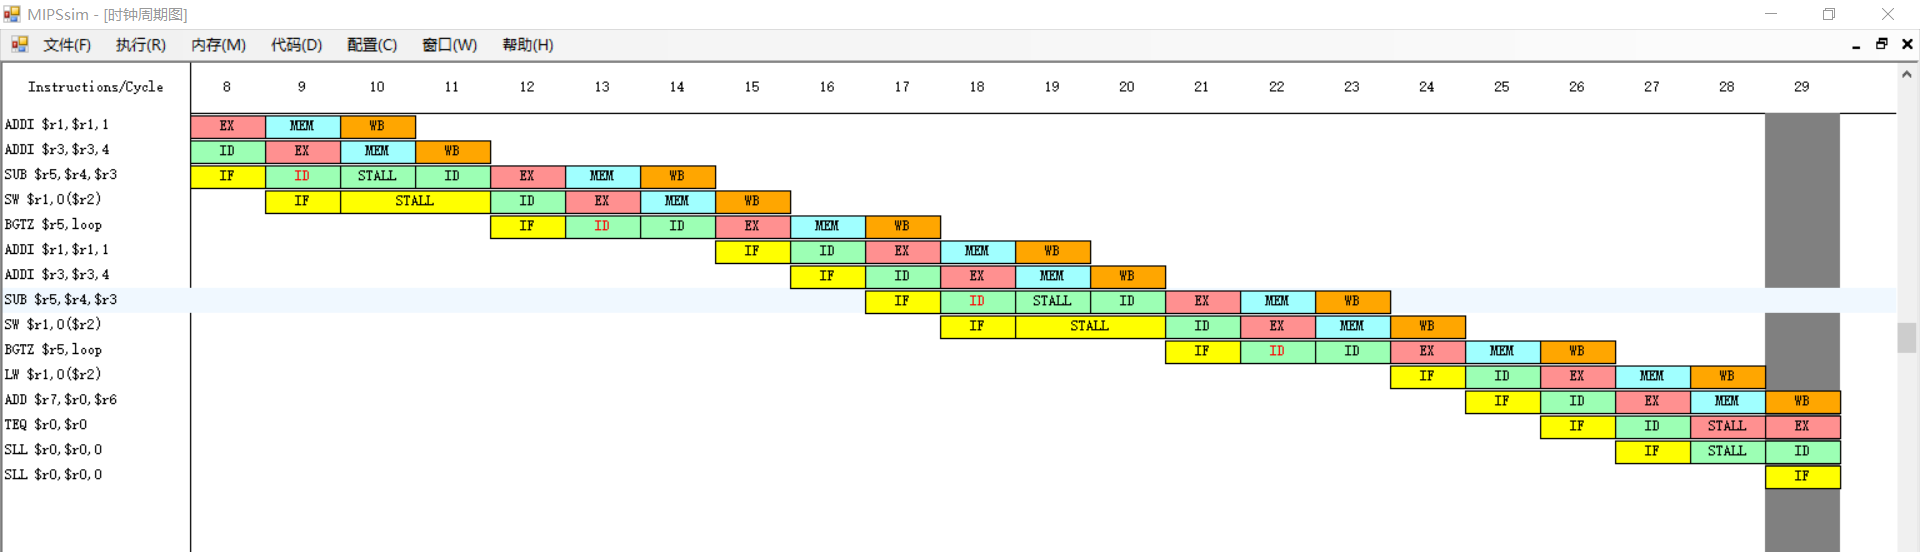
\includegraphics[width=.8\textwidth]{fig/delayed-branch.png}
                  \caption{时钟周期图}
                \end{figure}


        \end{itemize}

\end{enumerate}

\section{实验中的问题与心得}

实验中没有遇到任何问题。

本次实验的心得是,分支延迟作为 MIPS 当年提出时的特性之一,在大家都是顺序流水线时对性能做出了很好的优化。但是随着世代的更迭以及分支预测技术的逐渐成熟,到了上个世纪末分支延迟技术就成了 MIPS 前端性能的拖油瓶,现代的架构,例如 RISC-V 也都取消了这一设计。无论如何,我们尊重这一在当时有效的提升了性能的技术。

\end{document}